\chapter{沙箱实验与结果分析}\label{chap:exp}

% 说明实验环境
% - 硬件环境
% - 软件环境
% - 使用偏好(Master Node)
% 软硬件说明
% - redis、mysql
% 基准测试
% - 开销分析
% 不同内核配置实验
% 隔离性实验
%  - 资源限制效果说明
% 调度策略实验
%  - 互斥调度
% 
\section{实验环境}

实验环境有两台服务器构成,服务器硬件信息如表~\ref{tab:exp_env}所示。在CPU资源上,每台服务器上包含有两个Socket,单台总计80个物理核心,划分为4个Numa Node,同时,CPU均开启超线程,并使能Intel RDT,从而为可观测性基础设施提供末级缓存及内存带宽的监控,并为虚拟机提供按路数的末级缓存划分和固定补偿的内存带宽调控功能。在网络资源上,服务网卡支持SRIOV技术,能够为有网络性能需求的虚拟机提供硬件直通服务。

\begin{table}
    \bicaption{\quad 服务器硬件参数}{\quad Server Hardware Information}% caption
    \label{tab:exp_env}
    \footnotesize% fontsize
    \setlength{\tabcolsep}{4pt}% column separation
    \renewcommand{\arraystretch}{1.5}% row space 
    \centering
    \begin{tabular}{lc}
        \hline
        硬件资源 & 硬件信息 \\
        \hline
        CPU & Intel Xeon Gold 6148 (40 cores) * 2 \\
        Processor Core Frequency & 2.4GHz,Turbo 3.7 GHz \\
        L1 Caches & 32KB,  8-way set associative, split D/I \\
        L2 Caches & 1024KB, 16-way set associative \\
        L3 Caches & 28160KB, 11-way set associative \\
        Main Memory & 32GB * 8, 2666MHz DDR4 \\
        NIC & Intel Corporation Ethernet Connection X722 for 10GbE SFP+(10Gbit) \\
        \hline
    \end{tabular}
\end{table}

每台服务器的系统软件环境如表~\ref{tab:system_env}所示。在操作系统上,实验中选择使用较常见的Ubuntu22.04 LTS,Ubuntu同时也是Sched Ext优先支持的发行版,能够较方便地通过包管理工具安装预编译的Sched Ext内核。在虚拟换运行时上,Qemu采用发行版所支持的稳定版,而以轻量为目标的CloudHyeprvirsor则采用自编译的最新发布版本。

\begin{table}
    \bicaption{\quad 服务器系统环境}{\quad Server System Information}% caption
    \label{tab:system_env}
    \footnotesize% fontsize
    \setlength{\tabcolsep}{4pt}% column separation
    \renewcommand{\arraystretch}{1.5}% row space 
    \centering
    \begin{tabular}{lc}
        \hline
        软件类型 & 软件信息 \\
        \hline
        系统 & Ubuntu 22.04.3 LTS  \\
        内核 & 5.15.0-79-generic \\
        虚拟化运行时 & cloud-hypervisor v38.0-150 \\
                   & QEMU emulator version 6.2.0 \\
        其他        & libvirtd 8.0.0 \\
        \hline
    \end{tabular}
\end{table}

除系统软件之外,每台服务器还按照需要部署了其他关键服务。其中可观察基础设施按照第三章中所论述的架构进行搭建,Master节点上部署的了Prometheus与Grafana,用于进行数据采集与离线分析,Node节点上则部署的第三章中所提到的一系列Exporter,提供各个维度数据的采集能力。Master除对数据进行采集、存储、分析外,还额外部署了Harbor来对外提供容器管理服务,并承担大部分的配置文件存储。Node作为主要的实验场地,安装了Control Zone沙箱的所有相关的组件,并承担主要的服务运行。实验中对于Client-Server类型的任务,为尽可能地模拟真实环境,因此一般将Client放置在Master上。最后,实验中所涉及的关键服务都以容器镜像的形式分发并运行,因此在每个服务器上都需要安装容器运行时,而在容器运行时的选择上,对性能不敏感而对稳定性有要求的Master上使用Docker来提供容器服务,而在Node上,则使用Podman作为容器运行时,Podman相较Docker更加轻量,同时不存在Docker、Containerd等后台驻留服务,能够提供较为纯净的容器运行环境。

\section{沙箱性能实验}

Control Zone的启动开销计算从虚拟化运行时开始到系统引导至init过程的时间,虚拟机使用1CPU与512M内存的基础配置,在虚拟化运行时上,选择CloudHyperviosr与Qemu进行对比,而在精简内核上,选择Alpine Virt内核、Control Zone内核,以及CloudHyeprvirsor、Firecracker的默认精简内核,其中Alpine Virt内核为社区提供给云厂商的标准虚拟机内核,启动了大部分Guest优化功能,但同时也保留了对于众多设备的支持,而以轻量为目标的CloudHyeprvirsor、Firecracker也各自提供了默认的精简内核,相较于Alpine Virt内核,去除了大量无意义的驱动,几乎只支持virtio设备,其中CloudHypervisor默认内核还额外使能了PCI子系统,以便于使用SRIOV设备,实验中为了让实验结果更加具备可比性,因此使能了Firecracker内核中的PCI配置。

\begin{figure}[!htbp]
    \centering
    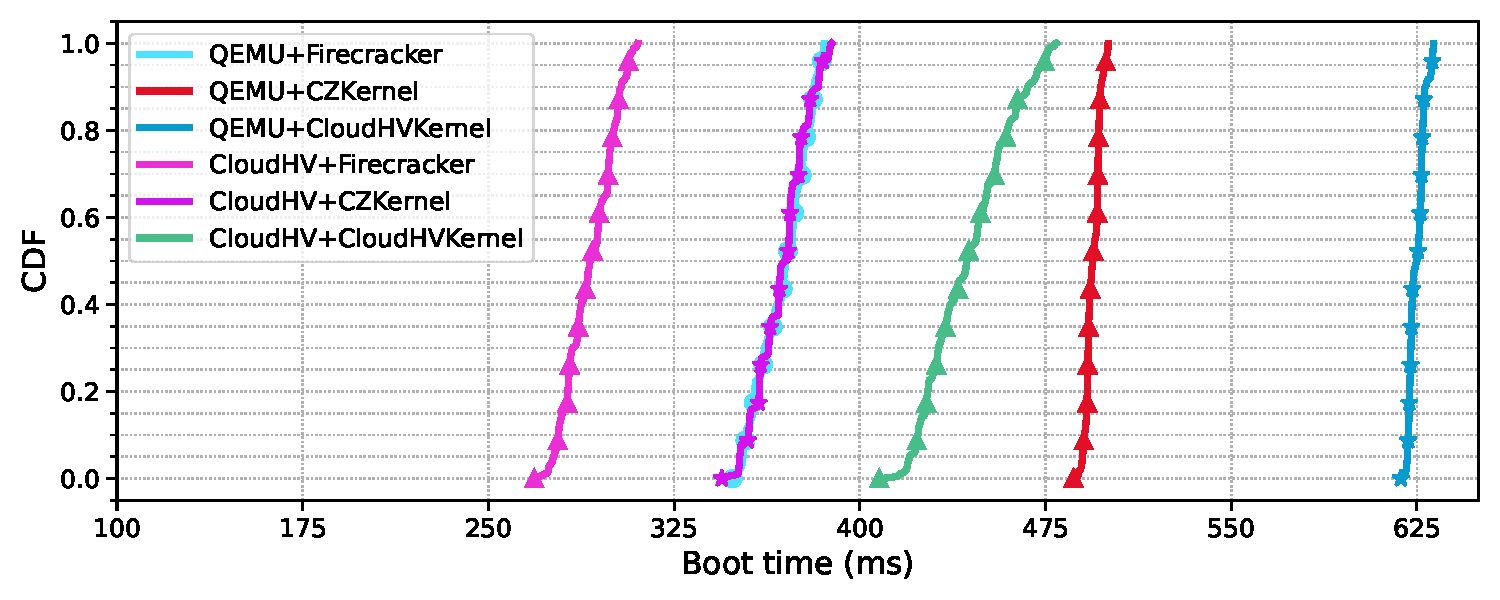
\includegraphics[width=0.8\textwidth]{boot_time_cdf}
    \bicaption{\quad Control Zone 、CloudHypervisor 及Firecracker内核的启动速度比较}{\quad The comparison of startup speed between Control Zone、CloudHypervisor and Firecracker.} 
    \label{fig:boot_time_cdf}
\end{figure}

实验结果如图~\ref{fig:avg_boot_time}所示,Control Zone内核的平均启动开销相较于Alpine Virt内核最高降低了88.8\%,对比不同的虚拟化运行时的数据发现而其中绝大部分的优化效果升来自于对内核的裁切,Control Zone内核仅支持运行容器、BPF子系统与Sched Ext调度类的最小功能,因此在启动时省去了大量非必要的工作,从而能够做到足够快速。同时还可以发现, 对于Alpine Virt内核而言,使用CloudHypervisor相较于Qemu降低28.9\%的启动时间,而观察两者的启动日志发现,虚拟化运行时所带来的提升主要来自于对于设备的裁切上,CloudHypervisor只需要针对云场景,因此相较于Qemu去除了大量的无关设备模拟,而更精简的设备一方面减少了虚拟化运行时的启动时间,另一方面,Guest内核也不必进行过多的设备探测与初始化,尤其在PCI子系统的初始化上,CloudHypervisor相较于Qemu,PCI子系统的初始化时间平均减少了83.2\%。相同的情况在其他内核上则有所不同,由于精简内核本身支持的设备驱动就十分有限,因此虚拟化运行时在这些内核的优化上主要体现在运行时启动本身上。

\begin{figure}[!htbp]
    \centering
    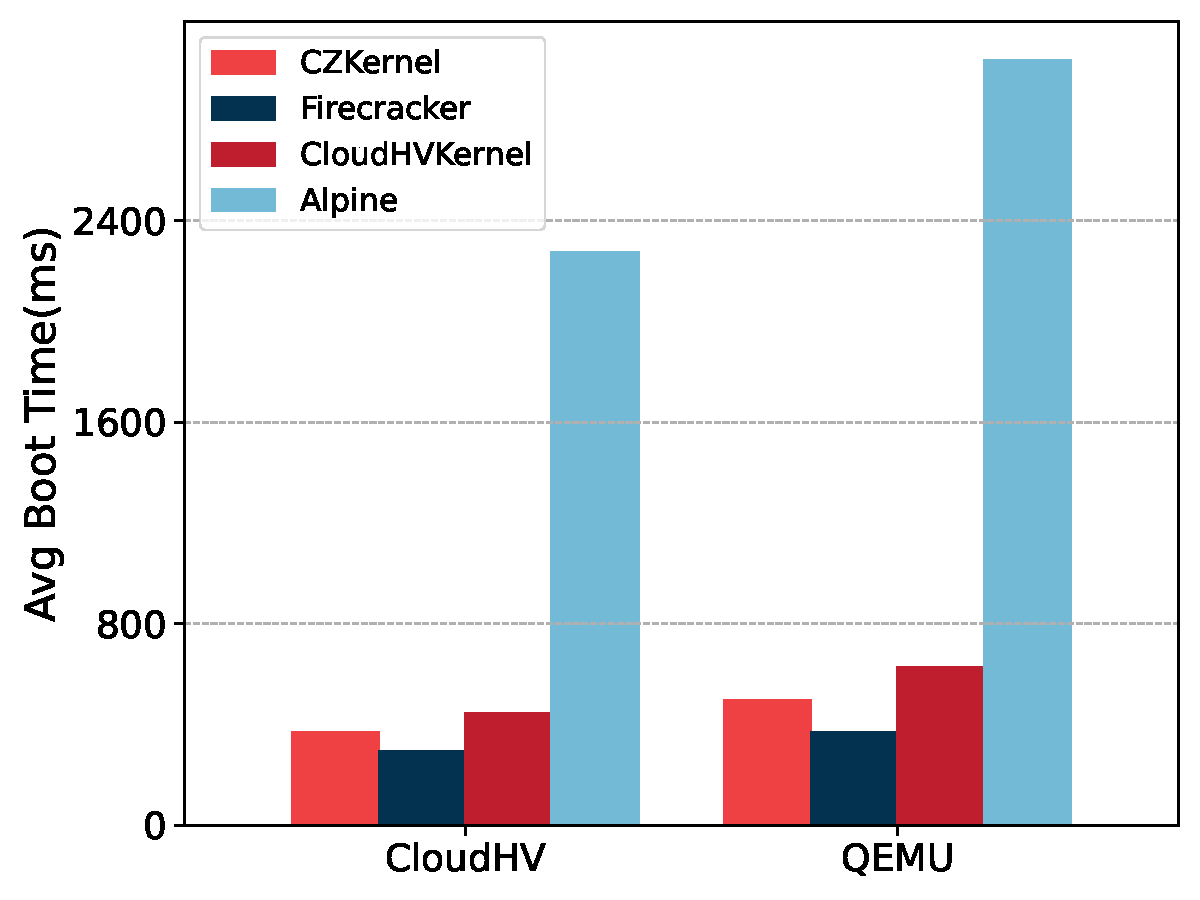
\includegraphics[width=0.7\textwidth]{avg_boot_time}
    \bicaption{\quad 启动时间为引导至运行init程序的时间,比较Firecracker(FC)、Control Zone(CZ)、Alpine(AL)内核,使用Cloud Hypervisor与Qemu}{\quad Boot time is the time it takes to boot to the init program. Compare Firecracker(FC), Control Zone(CZ), and Alpine(AL) kernels using Cloud Hypervisor and Qemu.}
    \label{fig:avg_boot_time}
\end{figure}

在精简内核的对比中,Control Zone内核也存在优势,如图~\ref{fig:boot_time_cdf}所示,使用Qemu时,Control Zone内核相较于CloudHypervisor默认内核在启动时间上减少了20.6\%,对比两者配置差异发现,CloudHypervisor所提供的精简内核虽然去掉了大部的驱动支持,但仍然保留了对嵌套虚拟化的支持而开启了虚拟化子系统,因此会产生额外的开销,而Control Zone内核所支持的容器环境所需要的支持则相对更少。但是相对于Firecra内核,Control Zone内核则在启动开销上并没有优势,即便使用Qemu虚拟化运行时,Firecracker内核也能达到接近使用CloudHypervisor的Control Zone内核的启动速度,比较配置能够发现, Firecracker内核在功能裁切上更加激进,分析两者的启动日志能够发现这开销的差异主要来自于Control Zone内核中所需要的额外功能,如Netfilter子系统等。这些功能在本设计中时必须的,同时考虑场景上的差异,Firecracker实现时希望以承担安全容器的运行时环境,虚拟机的生命周期与运行在其中的容器绑定,而在Control Zone的设计中,任务与Control Zone并非完全耦合,Control Zone更接近与对于隔离环境的声明,在任务需要运行时启动,而在任务运行完毕后仍然会保留,并提供给下一个任务使用,即Control Zone不会频繁地启动,因此这部分开销在设计中是可以接受的。

\section{定制内核性能实验}

\subsection{响应度优先}

% redis \ memcached

Control Zone响应度优先配置使用HZ\_1000配置时钟中断,并开启PREEMPT抢占模式。响应度优先内核的优势主要体现在多任务调度场景,因此在实验设计上,选择Redis、Memcached两种CPU敏感型应用来分别与CPU干扰应用混部以构造多任务场景,并使用CloudHypervisor默认提供的内核作为基准进行比较。实验在一个4CPU 512MB内存的Control Zone中进行。

\begin{figure}[H]
    \centering
    \begin{subfigure}[b]{0.45\textwidth}
      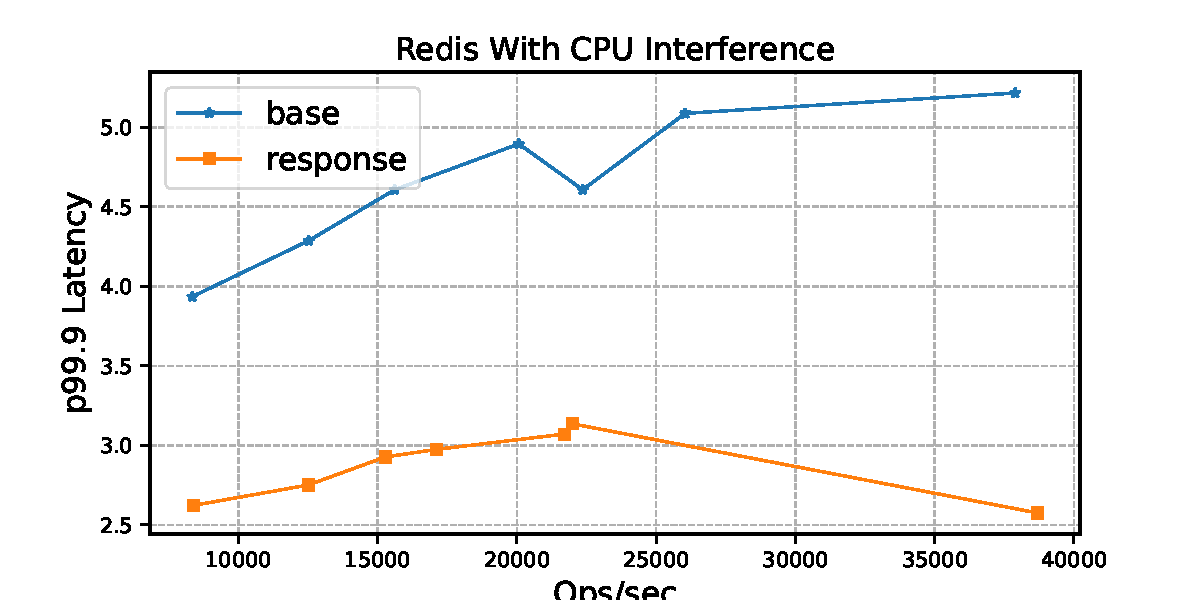
\includegraphics[width=\textwidth]{redis_response}
      \caption{Redis与干扰混部}
      \label{fig:redis_response}
    \end{subfigure}
    \begin{subfigure}[b]{0.45\textwidth}
      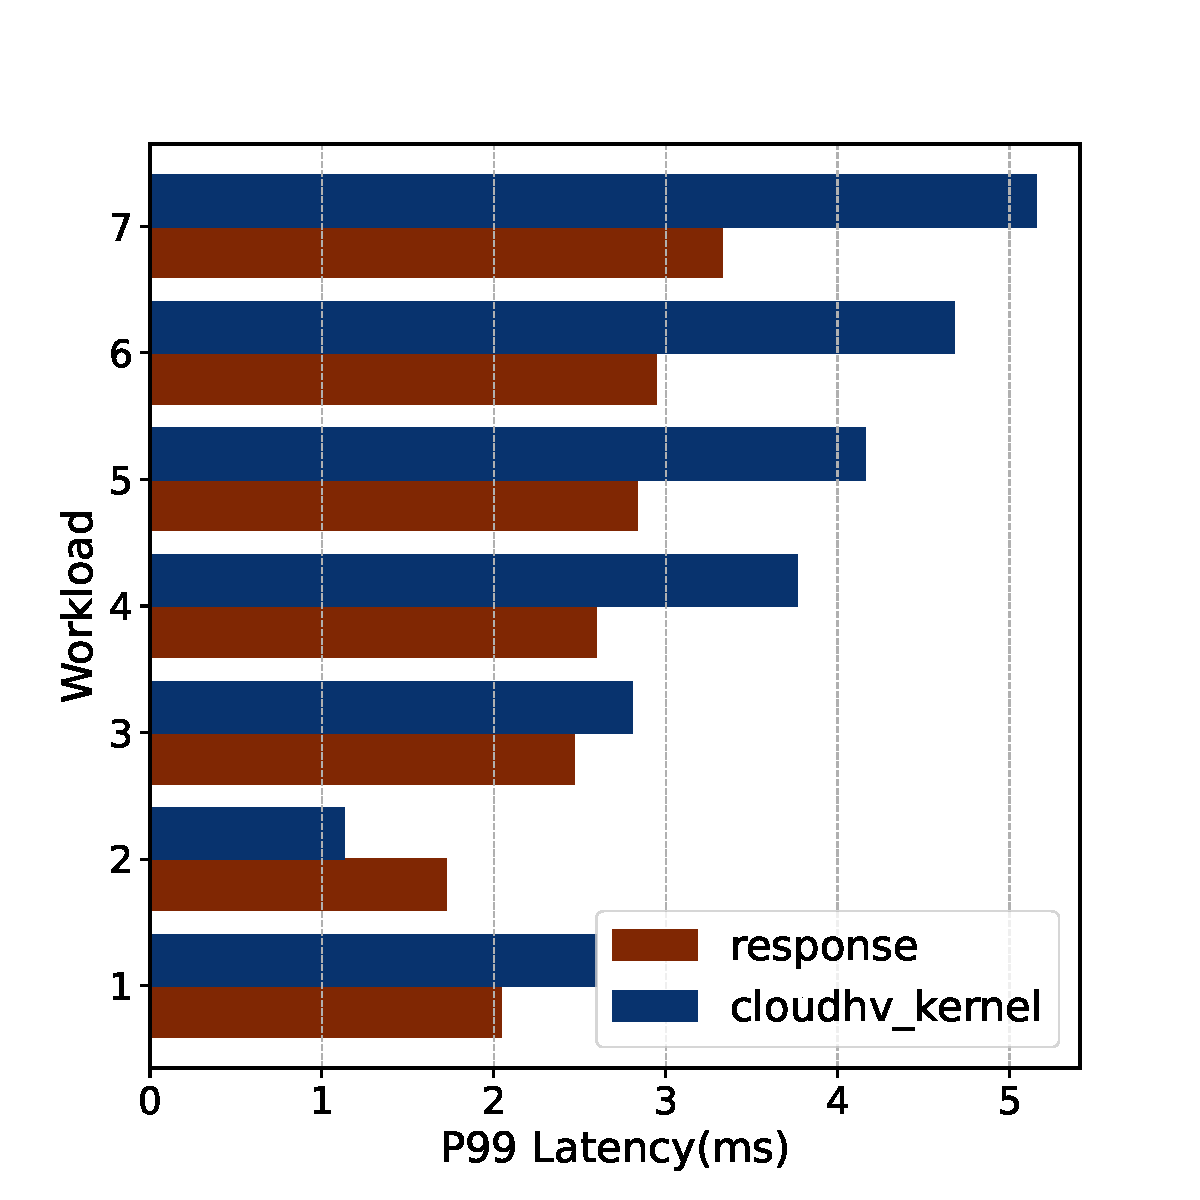
\includegraphics[width=\textwidth]{memcached_response}
      \caption{Memcached与干扰混部}
      \label{fig:memcached_response}
    \end{subfigure}
    \label{fig:lc_response}
  \end{figure}

混部实验结果如图~\ref{fig:lc_response}所示,在启用Control Zone响应度优先内核后,无论是Redis还是Memcached,在P99.9延迟上都要优于CloudHypervisor的默认内核,Reponse内核使用了更高的时钟中断频率,因此能够更快地在延时敏感应用与干扰应用中进行切换,同时在PREEMPT抢占模式下,网络中断能够更及时地进行处理,降低请求处理链路的整体延时。

\subsection{吞吐量优先}

% graph500(time) \ ffmjpeg 

Control Zone吞吐量优先配置使用HZ\_100配置时钟中断,并开启PREEMPT\_NONE抢占模式。吞吐量优先内核能够在任务量较少的场景中,让任务保持CPU资源的占用,从而更好地利用局部性,因此实验使用单一任务场景,选择Graph500作为目标应用,并对比其在CloudHypervisor默认内核、Throughput内核以及Response内核下的运行情况。实验在一个4CPU 512MB内存的Control Zone中进行。

\begin{figure}[!htbp][H]
    \centering
    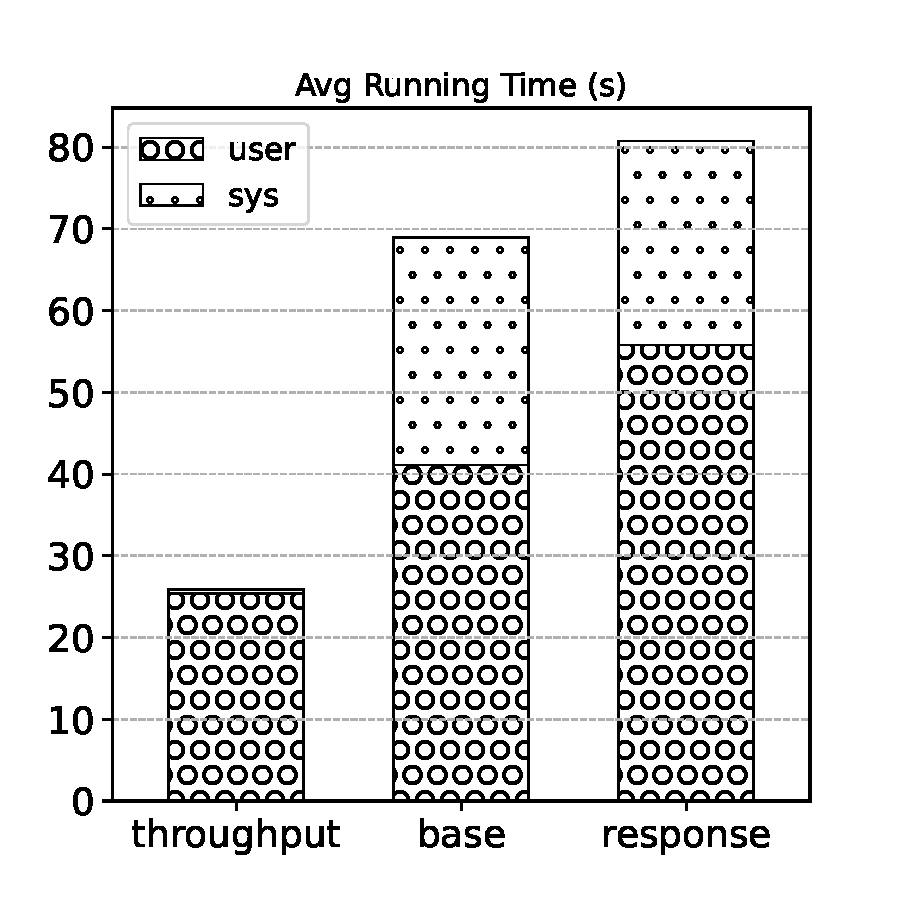
\includegraphics[width=0.8\textwidth]{avg_graph500_runtime}
    \bicaption{\quad 不同配置下的吞吐量差异}{\quad Throughput Discrepancy Across Different Configurations} 
    \label{fig:avg_graph500_runtime}
\end{figure}

Graph500主要执行图计算算法,因此执行时间是其重要的性能指标,实验中使用time工具记录任务的执行时间,包括用户态与内核态的执行时间, 具体实验结果如图~\ref{fig:avg_graph500_runtime}所示,其中使用Throughput内核的Control Zone消耗的时间最短,而使用Response内核的Control Zone则消耗的最长的时间,分析执行时间占比,在Throughput内核下,任务运行过程中内核态时间消耗几乎没有,而在Response内核中,内核态时间则占用了较大比例,造成这一结果的主要原因是时钟中断与NO_HZ配置,越高的时钟中断频率会引发越导致越频繁的陷入内核态,一方面使得内核态时间变得更长,另一方面也会导致局部性的破坏导致任务执行速度的减慢。

\section{BPF调度策略实验}

\subsection{强隔离调度策略}

% 增加调度策略的解释

BPF强隔离调度策略能够在混部场景中,为高优先级应用提供更好的性能保障,使得性能接近于无干扰的状态。而为验证强隔离调度策略的效果设计了两个混部场景的实验。场景一中使用4个独立的CPU,2048M内存的Control Zone进行实验,高优先级应用使用Mysql,而低优先级应用使用CPU干扰应用。场景二中则使用2CPU,512M的内存,并特别地使用SMT绑定为虚拟机CPU,同时选用延时敏感的Redis与CPU干扰进行混部。

混部场景一实验结果如图~\ref{fig:mysql_perf}所示,首先能够看出,Linux EEVDF调度器默认下以公平为目标,此时Mysql的性能并不能得到保障,而在降低CPU干扰应用的nice值之后,Mysql的性能虽然有一些提升,但相较于无干扰情况下仍存在较大劣化, 而分析Control Zone CPU使用率能够发现,Mysql在正常运行时并不会占用所有的核心,此时即便与干扰应用存在优先级上的差异,但由于这种优先级并不能跨越CPU调度队列产生效果,因此仍然存在一定程度上的并发,而由于资源竞争的Mysql的性能就会出现劣化。而在启用了BPF调度器之后Mysql性能几乎与没有干扰的情况下一致,首先,尽管优先级机制不能跨越核心产生作用,但在BPF调度器中能够自已强隔离的所里,使得高优先级的Mysql在运行时,低优先级的干扰应用能够自动的让出CPU,从而实现高优先级任务的性能保障。

\begin{figure}[!htbp]
    \centering
    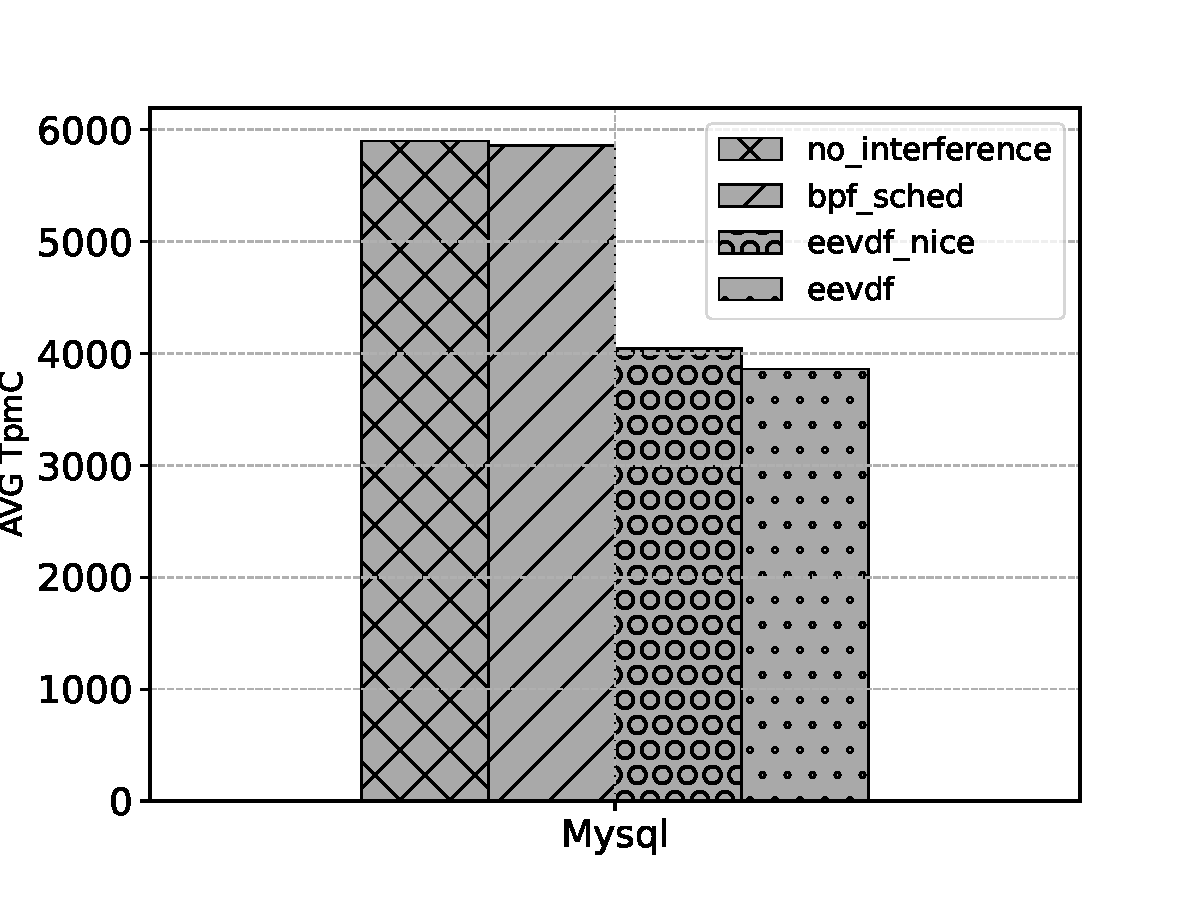
\includegraphics[width=0.8\textwidth]{mysql_perf}
    \bicaption{\quad Mysql与干扰混部}{\quad MySQL with Interference} 
    \label{fig:mysql_perf}
\end{figure}

混部场景二实验结果如图~\ref{fig:redis_smt}所示。SMT下Sibling共享了同一个物理CPU上的片上资源, 因此混部存在更激烈的资源竞争。Elfen\citep{yang2016elfen}通过修改内核与BE应用,使得BE应用能够主动探测Sibling上LC应用并及时出让CPU,从而保障LC应用的性能。这一策略对于SMT场景中的优先级应用性能保障来说十分重要,而受此启发的BPF强隔离调度策略能够在一定程度上达到类似的效果,而由于在探测频率上的差异,BPF强隔离机制还不能在SMT场景下完全保障高优先级任务的性能,但仍然强于Linux调度器。同时相较于Elfen,BPF Scheduler在开发与部署上都更加容易。

\begin{figure}[!htbp]
    \centering
    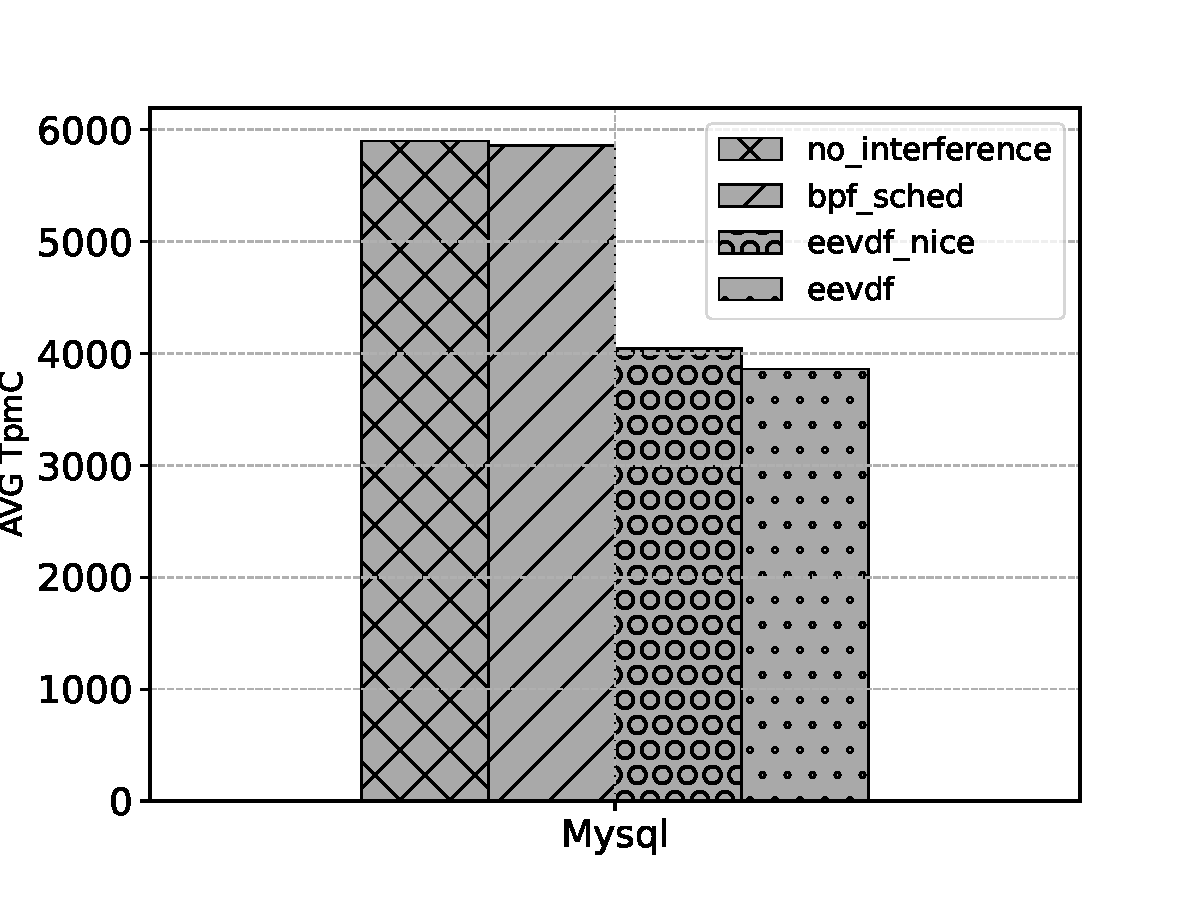
\includegraphics[width=0.8\textwidth]{mysql_perf}
    \bicaption{\quad SMT下Redis与干扰混部}{\quad Redis with Interference On SMT} 
    \label{fig:redis_smt}
\end{figure}

% \subsection{网络资源感知策略}

% \subsection{内存资源感知策略}
% Redis

\section{本章小结}

本章围绕Control Zone沙箱机制设计了一系列实验。首先,比较了Control Zone虚拟机的启动时间,通过在Hpervisor、Guest OS上的裁剪优化, Control Zone能够达到与领先轻量级虚拟化相近的水平。

随后,比较了不同内核下的应用性能,说明对于不同的应用而言,定制的内核能够在一定程度上提升其运行性能。最后,通过不同应用,不同硬件环境下的混部实验,说明了使用BPF Scheduler来针对不同的混部场景进行定制优化,在提升高优先级应用的性能保障效果上的优势。